%%%%%%%%%%%%%%%%%%%%%%%%%%%%%%%%%%%%%%%%%
% Beamer Presentation
% LaTeX Template
% Version 1.0 (10/11/12)
%
% This template has been downloaded from:
% http://www.LaTeXTemplates.com
%
% License:
% CC BY-NC-SA 3.0 (http://creativecommons.org/licenses/by-nc-sa/3.0/)
%
%%%%%%%%%%%%%%%%%%%%%%%%%%%%%%%%%%%%%%%%%

%----------------------------------------------------------------------------------------
%	PACKAGES AND THEMES
%----------------------------------------------------------------------------------------
\pdfminorversion=4

\documentclass[xcolor=table,compress]{beamer} %here use compress to have horizontal navigation bullets

\mode<presentation> {
\usetheme{Madrid}
\definecolor{myblue}{rgb}{0.19,0.55,0.91}
\colorlet{beamer@blendedblue}{myblue}
}

\usepackage{graphicx} % Allows including images
\usepackage{booktabs} % Allows the use of \toprule, \midrule and \bottomrule in tables
\usepackage{hyperref} % allow hyper links
\usepackage{color} % allow using colors

\usepackage{algorithm2e}
\usepackage{algorithmic}%
\usepackage{float}

\useoutertheme[subsection=false,shadow]{miniframes} %add navigation bullets

\definecolor{dgreen}{RGB}{0,128,0}
\definecolor{dred}{RGB}{255,0,0}
%----------------------------------------------------------------------------------------
%	TITLE PAGE
%----------------------------------------------------------------------------------------

\title[nextflow workshop 2018]{IARC nextflow pipelines: towards efficient cancer genomics analyses} 

\author{\textbf{Tiffany Delhomme}} % Your name
\institute[] % Your institution as it will appear on the bottom of every slide, may be shorthand to save space
{ \small PhD student at IARC(WHO) \\ \vspace*{0.25cm}
% Your institution for the title page
\medskip
\textit{} % Your email address
}
\date{22 nov. 2018} % Date, can be changed to a custom date

\begin{document}
\usebackgroundtemplate%
{%
    
\includegraphics[width=\paperwidth,height=\paperheight]{pictures/back_slide_1.pdf}%
}

\begin{frame}[noframenumbering]
\titlepage % Print the title page as the first slide
\end{frame}

\usebackgroundtemplate%
{%
    
\includegraphics[width=\paperwidth,height=\paperheight]{pictures/back_all_slides.pdf}%
}
%----------------------------------------------------------------------------------------
%	PRESENTATION SLIDES
%----------------------------------------------------------------------------------------
\small
\begin{frame}{Presentation}{Who Am I?}
\begin{itemize}
	\item \textit{M.D} Evolution, Bioinfo, Biomaths from Universite Lyon 1, France (2014)
	\item \textit{M.D} Theoretical Computer Science - Complex Systems from ENS Lyon and IXXI institute, France (2015)
	\item \textbf{current}: 4th year PhD student in Bioinformatics and Cancer Genomics at IARC, Lyon, France
	\begin{itemize}
		\item \textit{Dealing with NGS errors to produce efficient variant calling. Application to early cancer detection.}
	\end{itemize}
\end{itemize}
\end{frame}

\begin{frame}{Presentation}{IARC Lyon}
International Agency for Research on Cancer (IARC)
\begin{tabular}{cl}  
	\begin{tabular}{c}
		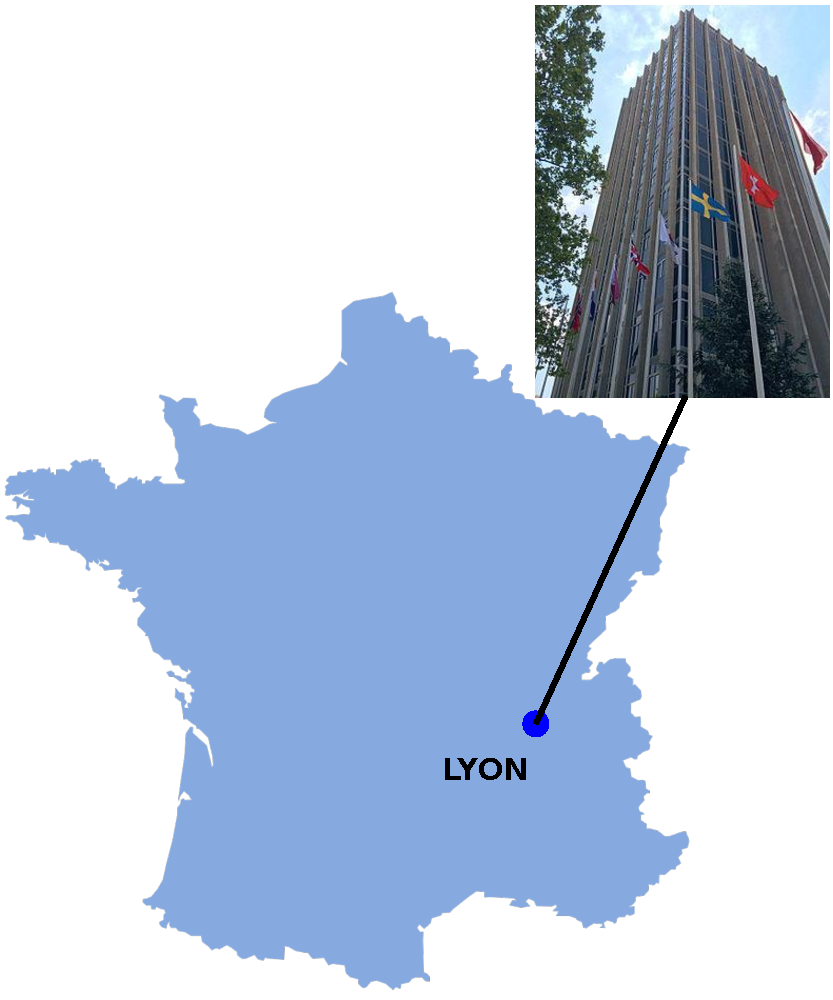
\includegraphics[scale=0.4]{pictures/map_iarc.pdf}
	\end{tabular}
    & \begin{tabular}{l}
	\parbox{0.45\linewidth}{%  change the parbox width as appropiate
	\pause 
	\begin{itemize}
		\item Created in 1965, intergovernmental agency forming part of the World Health Organization \pause
		\item Mostly known for:
				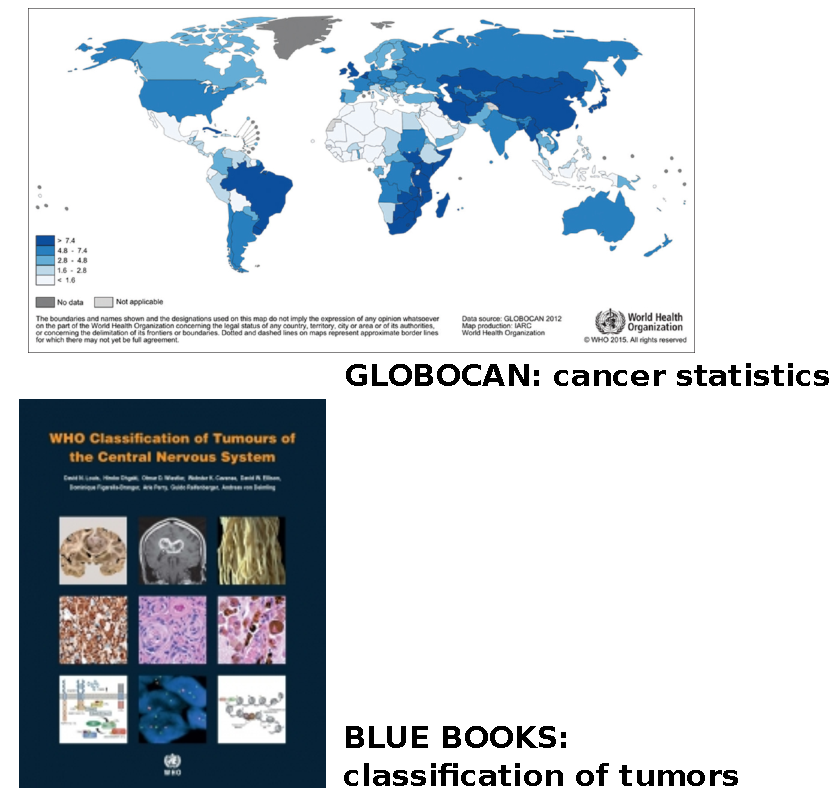
\includegraphics[scale=0.3]{pictures/known2.pdf}
	\end{itemize}
	}
	\end{tabular}
\end{tabular}
\end{frame}

\begin{frame}{Cancer genomics at IARC}{Multiple teams, multiple projects}
\pause \vspace*{-0.5cm}
\begin{center}
\only<2>{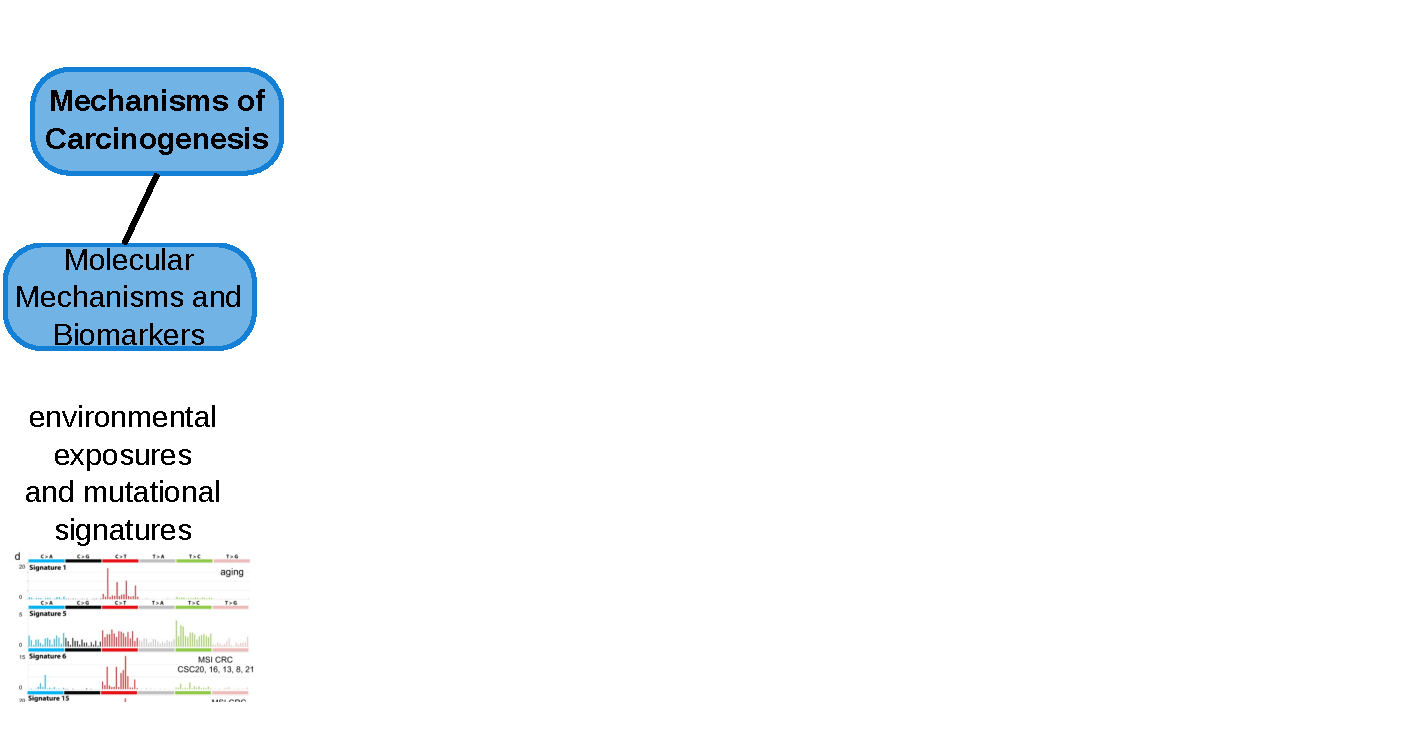
\includegraphics[scale=0.5]{pictures/genomics1.pdf}}
\only<3>{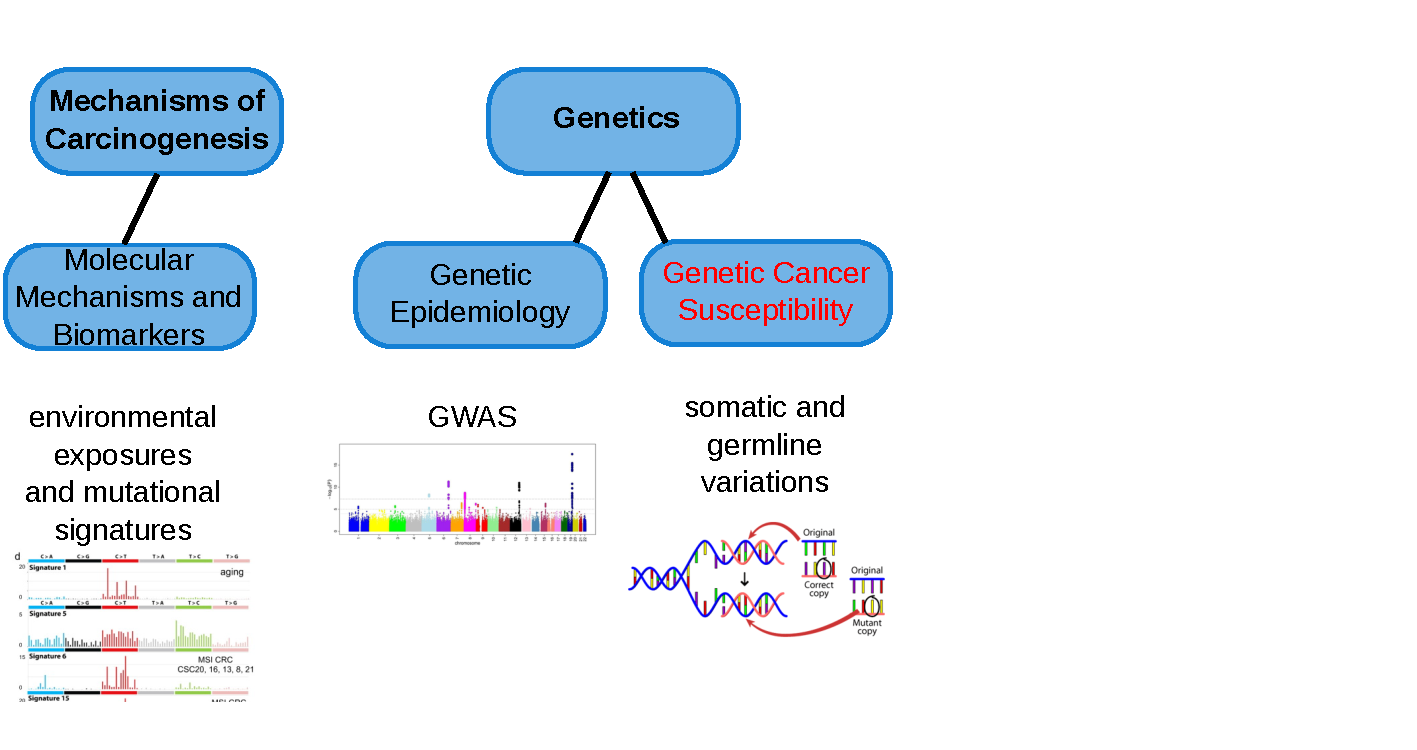
\includegraphics[scale=0.5]{pictures/genomics2.pdf}}
\only<4>{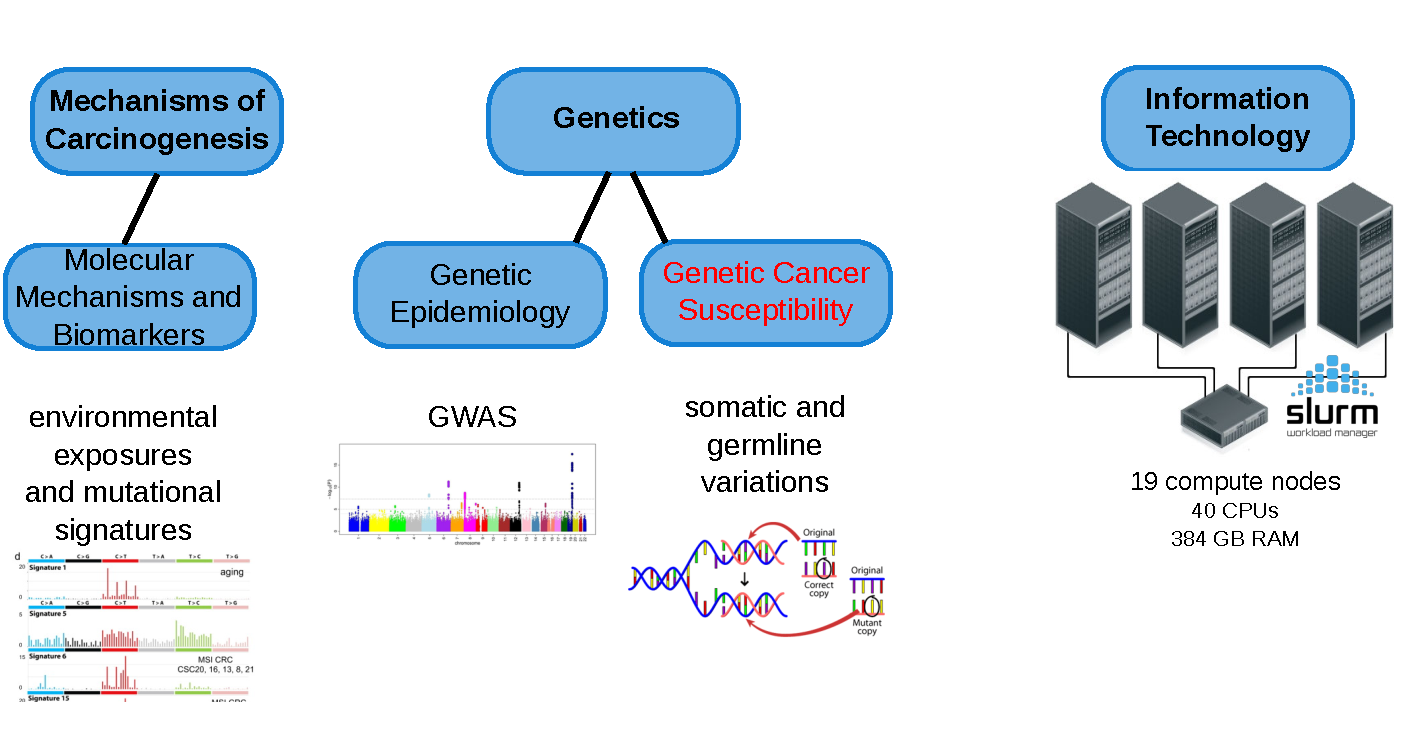
\includegraphics[scale=0.5]{pictures/genomics.pdf}}
\end{center}
\end{frame}

\begin{frame}{Why nextflow?}{For cancer genomics analyses}
Nextflow enables scientists to write workflow emphasizing on:
\begin{itemize}
	\item \textbf{efficiency}: parallel computations $\Rightarrow$ analyses of hundreds of cancer genomes \pause
	\item \textbf{robustness}: scalable computations $\Rightarrow$ multiple HPC environments + local machines \pause
	\item \textbf{reproducibility}: GitHub + Docker + Singularity $\Rightarrow$ n-uplication of analyses, validations \pause
	\item \textbf{user-friendliness}: 1 command line, no software installation $\Rightarrow$ user profile palette is large (biologists, students, pathologists,...)
\end{itemize}
\end{frame}

\begin{frame}{Implementation pattern}{Efficiency, robustness, user-friendliness and reproducibility}
\begin{center}
\only<1>{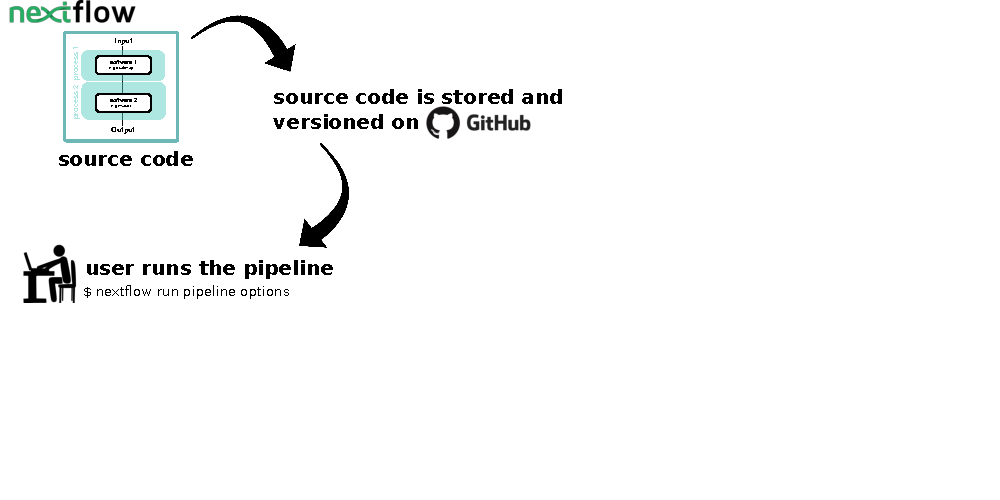
\includegraphics[scale=0.7]{pictures/pipelines1.pdf}}
\only<2>{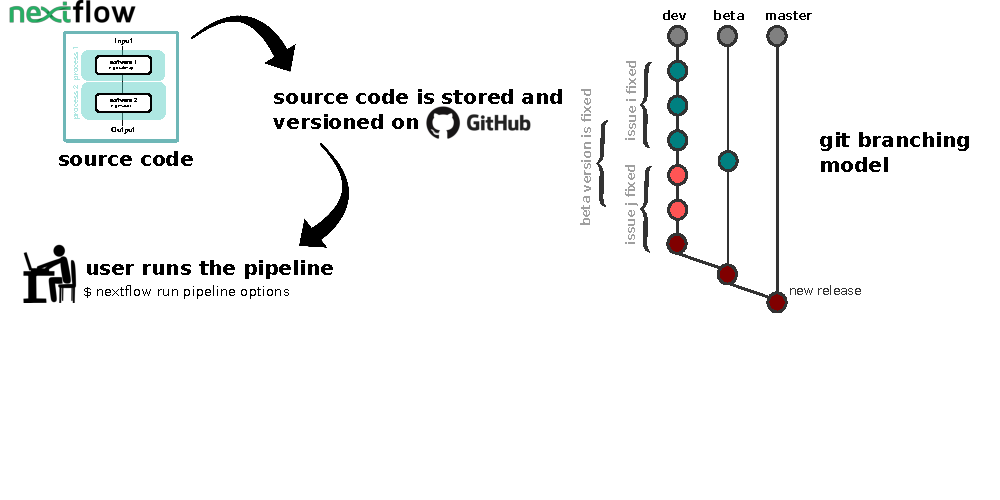
\includegraphics[scale=0.7]{pictures/pipelines2.pdf}}
\only<3>{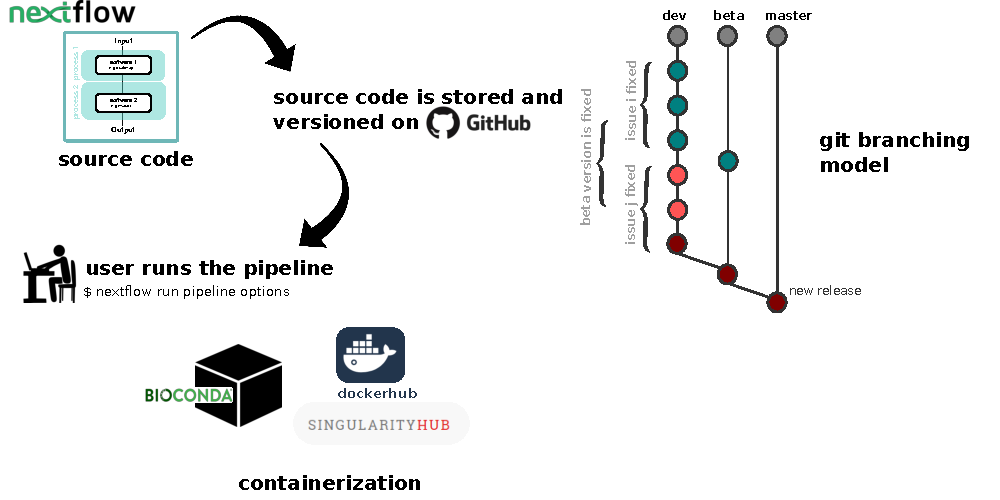
\includegraphics[scale=0.7]{pictures/pipelines3.pdf}}
\only<4>{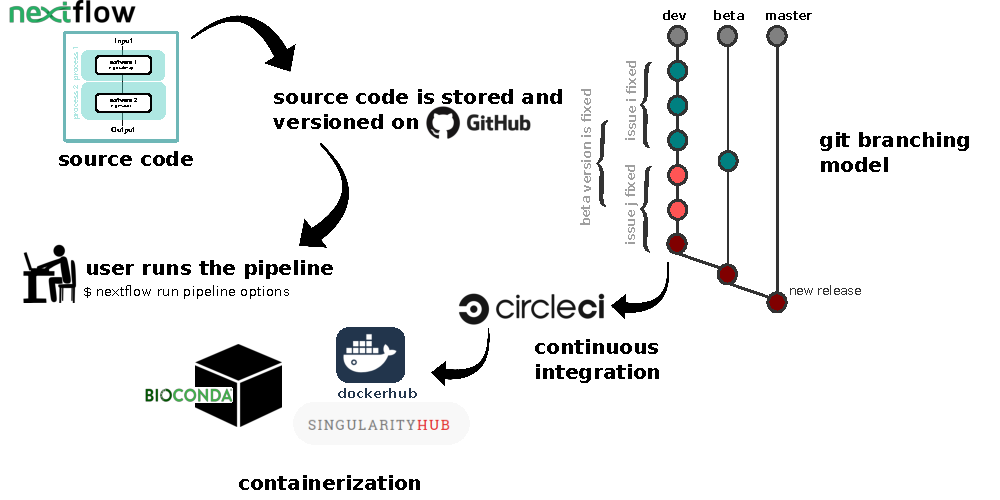
\includegraphics[scale=0.7]{pictures/pipelines.pdf}}
\end{center}
\end{frame}

\begin{frame}{GitHub IARCbionfo}{open-source pipelines}
\href{https://github.com/IARCbioinfo}{\beamergotobutton{GitHub webpage}} \end{frame}

\begin{frame}{ITH pipeline example}{Intra-tumor heterogeneity leads to multiple subclones}
Genetic variation within individual tumors (ITH) provides insights into: \vspace*{-0.15cm}
\begin{itemize}
	\item cancer evolutionary trajectories \vspace*{-0.2cm}
	\item cancer resistance to therapies \vspace*{-0.2cm}
	\item cancer molecular classifications \pause
\end{itemize}
\begin{center}
	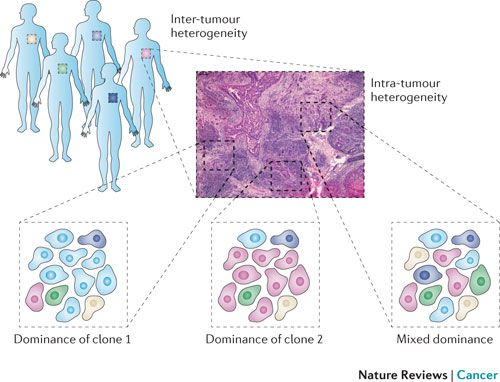
\includegraphics[scale=0.4]{pictures/ITH_clinics.jpg} \\
\end{center}
\end{frame}

\begin{frame}{ITH pipeline example}{In practice (with L. Soudade and I. Lboukili)}
\begin{center} 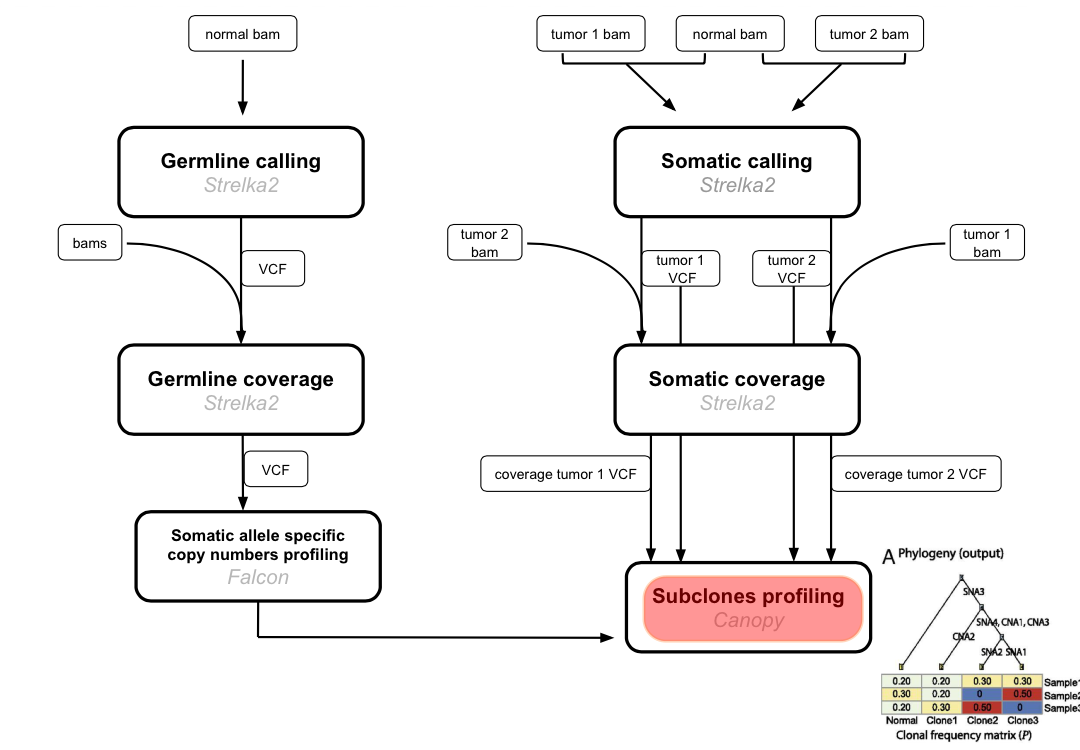
\includegraphics[scale=0.25]{pictures/ITH-nf.png} \end{center}
\end{frame}

\begin{frame}{Acknowledgements}
\begin{center}
	
\includegraphics[scale=0.2]{pictures/thanks.pdf} \\
\end{center}
\end{frame}

\end{document}